% This is LLNCS.DOC the documentation file of
% the LaTeX2e class from Springer-Verlag
% for Lecture Notes in Computer Science, version 2.4
\documentclass{article}

\usepackage{cite}
\usepackage{listings}
\usepackage{amssymb}
\usepackage{mathpartir}
\usepackage{amsmath}    
\usepackage{algpseudocode}
\usepackage{array}
\usepackage{xcolor}
\usepackage{fullpage}
\usepackage{graphicx}
\linespread{1.2}

\usepackage{hyperref}
\hypersetup{
    colorlinks=true,
    linkcolor=blue,
    filecolor=magenta,      
    urlcolor=cyan,
}
 
\urlstyle{same}

\lstset{
    string=[s]{"}{"},
    stringstyle=\color{blue},
    comment=[l]{:},
    commentstyle=\color{black},
}


\begin{document}
\title{Translating the JSON Representation of CoCoSim Models to Lustre Programs}

\author{Baoluo Meng}


\maketitle

This is to document the translation from the JSON representation of a CoCoSim model to its semantic equivalent representation in Lustre.


\section{JSON Representation of CoCoSim Models}


CoCoSim supports a subset of the blocks provided by the Simulink toolset. 
A CoCoSim model is a visualization of a set of Simulink blocks declarations, their connectivities and Stateflows.
The translation supports a subset of CoCoSim functional blocks including Vector Concatenate, Selector, Constant, Data Type Conversion, Demux, Logic, Math, MinMax, Mux, Product, Relational Operator, Rounding, Sum, Switch and UnitDelay. 
In addition to the list of functional blocks, we extends Simulink with contract blocks to allow modeling \textsf{assume, guarantee, mode, requires} and \textsf{ensures}, which are essentially Subsystem blocks in Simulink. 
One of the goals of CoCoSim is to verify properties about the model. 
A property is encoded in \textsf{Observer} block, which is a subsystem block in Simulink. 

The front end of CoCoSim translates a CoCoSim model to an intermediate representation in JSON. 
The root of the JSON file consists of meta information about the model including the file path, the sample time of the CoCoSim model and the date of the model generated, and the definition of top-level block.
The top-level block definition is defined as a pair of block identifier and a value, where value stores its content information.


Below shows the JSON schema for the intermediate representation of a CoCoSim model consisting of meta information, block content definition, and Stateflow content definition.
We will discuss block content and Stateflow content definitions in the following two sections.

\small{
\begingroup\makeatletter\def\@currenvir{verbatim}
\verbatim
{
    "$schema": "http://json-schema.org/draft-06/schema#",
    "title": "IR Schema",
    "description": "The JSON representation of a CoCoSim model",
    "type": "object",
    "properties": {
        "meta": {
            "description": "Meta information about the JSON file",
            "properties": {
                "file_path": {
                    "type": "string"
                },
                "sampleTime": {
                    "type": "integer"
                },
                "date": {
                    "type": "string"
                }
            }
        }
    },
    "additionalProperties": { 
        "type": "object",
        "properties": {
            "Content": {"$ref": "#/definitions/content"}
        },
        "minProperties": 0,
        "maxProperties": 1        
    },
    "definitions": {
       "block" : {
          "description": "The JSON representation of a CoCoSim block",
          "type": "object",
          "properties": {
              "Handle": {
                  "type": "number"
              },   
              "Name": {
                  "type": "string"
              },    
              "Path": {
                  "type": "string"
              },   
              "Port": {
                  "type": "integer"
              },         
              "Origin_path": {
                  "type": "string"
              },  
              "PortConnectivity": {
                  "properties":{
                      "SrcBlock": {
                          "type": "array",
                          "items": {"type":"number"}
                      },
                      "DstBlock": {
                          "type": "array",
                          "items": {"type":"number"}
                      }
                  }
              },                                          
              "Criteria": {
                  "type": "string",
                  "enum": ["u2 >= Threshold", "u2 > Threshold", "u2 ~= 0"]
              },
              "Value": {
                  "type": "string"
              },                
              "Operator": {
                  "type": "string",
                  "enum": ["NOT", "AND", "OR", "XOR", 
                           "NAND", "NOR", "NXOR",
                           "==", ">=", ">", "<=", "<", 
                           "?=", "?", "Floor", "Ceil", 
                           "Round", "Fix"]
              },
              "ContractBlockType": {
                  "type": "string",
                  "enum": ["ContractGuaranteeBlock", "ContractModeBlock", 
                           "ContractAssumeBlock", "ContractRequireBlock", 
                           "ContractEnsureBlock"]
              },                
              "BlockType": {
                  "type": "string",
                  "enum": ["Inport", "Outport", "Subsystem", "Constant", 
                           "Memory", "UnitDelay", "Switch", "Product",
                           "RelationalOperator", "Logic", "MinMax", "Sum", 
                           "UnaryMinus", "DataTypeConversion", "Rounding", 
                           "VectorConcatenation", "Mux", "Demux"]
              },
              "CompiledPortDataTypes": {
                  "properties":{
                      "Inport": {
                          "type": "string",
                          "enum": ["double", "single", "int8", "uint8", 
                                   "int16", "uint16", "int32", "uint32"]                    
                      },
                      "Outport": {
                          "type": "string",
                          "enum": ["double", "single", "int8", "uint8", 
                                   "int16", "uint16", "int32", "uint32"]                                       
                      }
                  }            
              },
              "CompiledPortDimensions": {
                  "properties":{
                      "Inport": {
                          "type": "array",
                          "items": {
                              "type": "integer"
                          }                             
                      },
                      "Outport": {
                          "type": "array",
                          "items": {
                              "type": "integer"
                          }                             
                      }
                  }             
              },        
              "Content": {
                  "$ref": "#/definitions/content"
              },
              "StateflowContent": {
                  "$ref": "#/definitions/stateflowcontent"}
              }             
          },
          "stateflowcontent": {
            "type": "object",
            "properties": {
                "Name": {
                    "type": "string"
                },    
                "Path": {
                    "type": "string"
                },   
                "Data": {
                    "type": "array",
                    "items": {
                        "type": "object",
                        "properties": {
                            "Id":{
                                "type": "string"
                            }, 
                            "Name":{
                                "type": "string"
                            },
                            "CompiledType":{
                                "type": "string",
                                "enum": ["double", "single", "int8", "uint8", 
                                            "int16", "uint16", "int32", "uint32"]                    
                            },
                            "Port":{
                                "type": "integer"
                            },                  
                            "Scope":{
                                "type": "string",
                                "enum": ["Input", "Local", "Output"]                    
                            }                                                                                 
                        }
                    }
                },         
                "States": {
                    "type": "array",
                    "items": {
                        "type": "object",
                        "properties": {
                            "Id":{
                                "type": "string"
                            }, 
                            "Path":{
                                "type": "string"
                            },
                            "Name":{
                                "type": "string"
                            },                    
                            "Actions":{
                                "type": "object",
                                "properties": {
                                    "Entry": {
                                        "type": "string"
                                    },
                                    "During": {
                                        "type": "string"
                                    },
                                    "Exit": {
                                        "type": "string"
                                    }                                                        
                                }                  
                            },
                            "OuterTransitions":{
                                "type": "array",
                                "items": {
                                    "type": "object",
                                    "properties": {
                                        "Destination":{
                                            "type": "array",
                                            "items": {
                                                "type": "object",
                                                "properties": {
                                                    "Id":{
                                                        "type": "string"
                                                    }, 
                                                    "Destination":{
                                                        "properties": {
                                                            "Id": {
                                                                "type": "string"
                                                            },
                                                            "Type": {
                                                                "type": "string",
                                                                "enum": ["State", "Junction"]
                                                            }
                                                        }
                                                    },
                                                    "Condition":{
                                                        "type": "string"
                                                    },
                                                    "ConditionAction":{
                                                        "type": "string"
                                                    },                  
                                                    "TransitionAction":{
                                                        "type": "string"                   
                                                    }                                                                                 
                                                }
                                            }
                                        }                                                                               
                                    }
                                }
                            },                  
                            "Composition":{
                                "type": "object",
                                "properties": {
                                    "Type": {
                                        "type": "string",
                                        "enum": ["EXCLUSIVE_OR", "PARALLEL_AND"]
                                    },
                                    "Substates": {
                                        "type": "array",
                                        "items": {
                                            "type": "string"
                                        }
                                    },
                                    "States": {
                                        "type": "number"
                                    },
                                    "DefaultTransitions": {
                                        "type": "object",
                                        "properties": {
                                            "Id": {
                                                "type": "string"
                                            },
                                            "Destination": {
                                                "type": "object",
                                                "properties": {
                                                    "Id": {
                                                        "type": "string"
                                                    },
                                                    "Name": {
                                                        "type": "string"
                                                    },                                            
                                                    "Type": {
                                                        "type": "string",
                                                        "enum": ["State", "Junction"]
                                                    }                                            
                                                }
                                            },
                                            "Condition":{
                                                "type": "string"
                                            },
                                            "ConditionAction":{
                                                "type": "string"
                                            },                  
                                            "TransitionAction":{
                                                "type": "string"                   
                                            }                                      
                                        }
                                    }
                                }                  
                            }                                                                                 
                        }
                    }
                },         
                "CompiledPortDataTypes": {
                    "properties":{
                        "Inport": {
                            "type": "string",
                            "enum": ["double", "single", "int8", "uint8", 
                                        "int16", "uint16", "int32", "uint32"]                    
                        },
                        "Outport": {
                            "type": "string",
                            "enum": ["double", "single", "int8", "uint8", 
                                        "int16", "uint16", "int32", "uint32"]                                       
                        }
                    }            
                },
                "CompiledPortDimensions": {
                    "properties":{
                        "Inport": {
                            "type": "array",
                            "items": {
                                "type": "integer"
                            }                             
                        },
                        "Outport": {
                            "type": "array",
                            "items": {
                                "type": "integer"
                            }                             
                        }
                    }             
                }     
            }           
        },
        "content" : {
            "type": "object",
            "additionalProperties": {"$ref": "#/definitions/block"}
        }          
    },
    "required": ["meta"]
}
\end{verbatim}
}

\subsection{CoCoSim Blocks in JSON}

%The CoCoSim intermediate compiler takes as input a Simulink model and translate it into a JSON representation storing blocks and connectivities information. 
%The model information is stored as block name -- value pairs in a JSON file. 
%The name field specifies the name of the block, and the value stores the actual data about the block such as block handle, block connectivities and so on. 
Each block is uniquely identified by its block handle.
The \textsf{``BlockType"} field specifies the type of a block. 
%For example, an inport block of a CoCoSim model has a ``BlockType" ``Inport".
The blocks connectivity information is stored in the \textsf{``PortConnectivity"} field, where \textsf{``SrcBlock"} stores the handles of incoming blocks, whereas \textsf{``DstBlock"} stores the handles of destination blocks. 
The \textsf{``Origin\_path"} is the full path to the block in the CoCoSim model.
The value of \textsf{``Port"} of inports or outports is the position index in the inputs or outputs. 

Figure~\ref{cocosimmodel} shows an overview of a CoCoSim model ``unsafe\_1\_PP" and Figure~\ref{jsoninport} shows a snippet of its JSON representation. 
\textsf{``In1"} and \textsf{``In2"} are the names of the inport blocks; \textsf{``Inport"} is the type of block \textsf{``In1"}; and the handle is \textsf{``77.0003662109375"}, which is the unique identifier for \textsf{``In1"}. 
\textsf{``Out1"} is the outport of the block.
The data type of \textsf{``In1"} is stored in the attribute \textsf{``Outport"} of \textsf{``CompiledPortDataTypes"}, which is Boolean. 
Since \textsf{``In1"} is an inport of top most node, it only has destination blocks. 
The handles of its destination blocks are store as values \textsf{\{79.0003662109375, 92.0008544921875\}} in \textsf{``DstBlock"} of \textsf{``PortConnectivity"}. 
The \textsf{``Origin\_path"} of \textsf{``In1"} is \textsf{``unsafe\_1\_PP/In1"}.
\textsf{``In1"} has a ports value of 1, meaning it is the first input. 
Subsystem is a type of \textsf{subsystem}, which defines the relations among \textsf{``In1", ``In2"}, and \textsf{``Out1"}. 
Safety is an observer block that defines a property in terms of inputs and outputs of the subsystem block ``unsafe\_1\_PP". 
Safety\_term is a terminator block.

Figure~\ref{jsonsafety} shows a snippet of the observer block ``safety" in JSON, which is a type of subsystem block with the annotation type \textsf{``ensures"}.
It connects with \textsf{``SrcBlock"} with handles\textsf{ \{77.0003662109375, 78.0003662109375, 920008544921875\}}, which are the handles of inports \textsf{``In1"} and \textsf{``In2"} and outport \textsf{``Out1"} of the calling node \textsf{``unsafe\_1\_PP"},  and connects with \textsf{``DstBlock"} with handle \textsf{``91.000732421875"}, which is the handle of the terminator block \textsf{``Safety\_term"}. 

Figure~\ref{cocosimsafety} shows the CoCoSim model of the observer block \textsf{``Safety"} and Figure~\ref{jsonsafetybody} shows the definition of the observer block body in JSON, including 
three inports \textsf{``In1", ``In2"}, and \textsf{``Out1"}, an outport \textsf{``Safety"}, a logical operator \textsf{``AND"}, and a relational operator \textsf{``$>=$"}. 
Based on the connectivities defined in the port connectivity, \textsf{``Safety"} connects with the source block logical operator \textsf{``AND"}, the logical operator \textsf{``AND"} connects with the source blocks relational operator \textsf{``$>=$"} and the inport block \textsf{``Out1"}, and the relational operator \textsf{``$>=$"} connects
with the source block inports \textsf{``In1"} and \textsf{``In2"}. 
They all together comprise the expression: \textsf{Safety = Out1 AND (In1 $>=$ In2)}.

\begin{figure}[h]
\begin{center}
    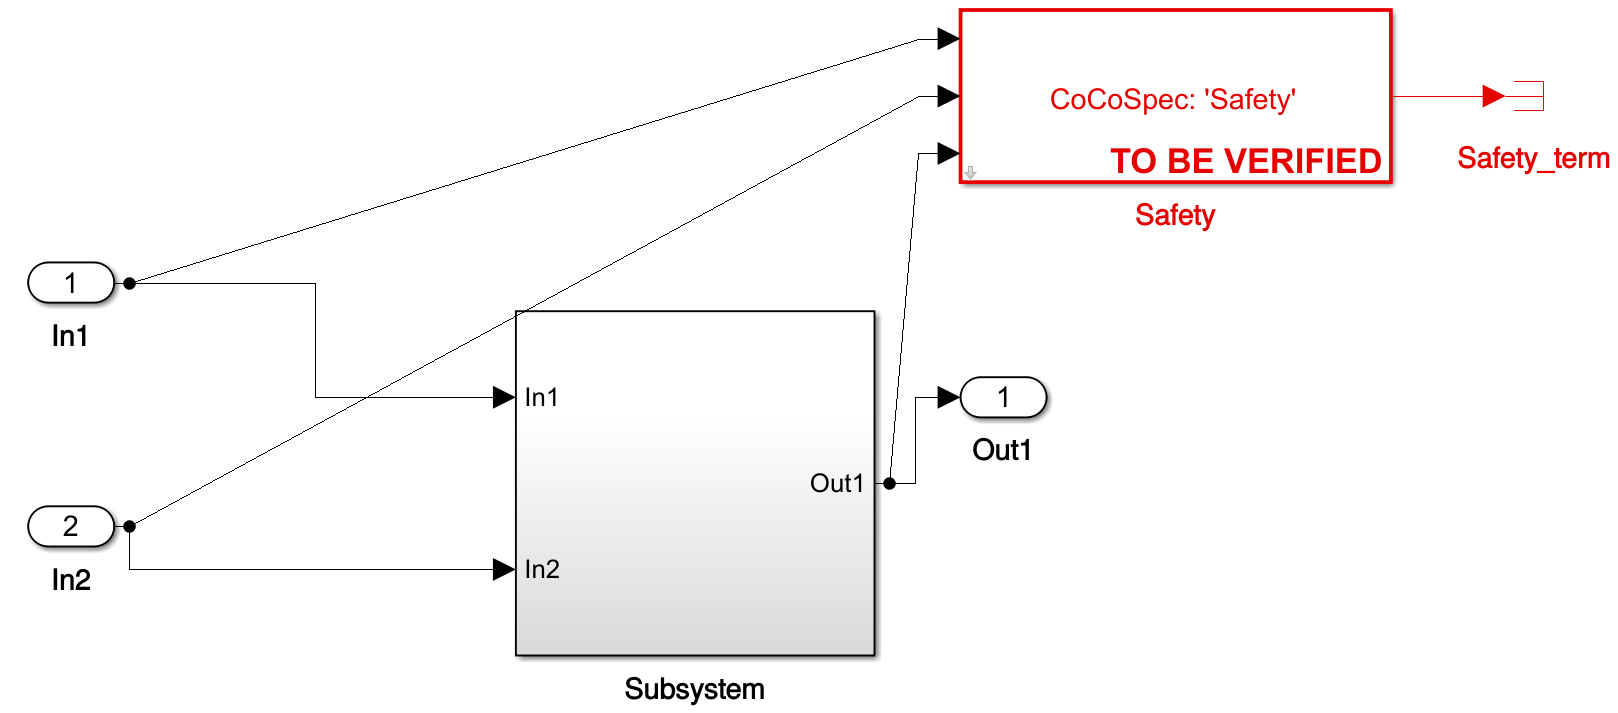
\includegraphics[scale=0.2]{figures/safety000}
\end{center}  
  \caption{A CoCoSim Model}
  \label{cocosimmodel}
\end{figure}

\begin{figure}[h]
\begin{center}
  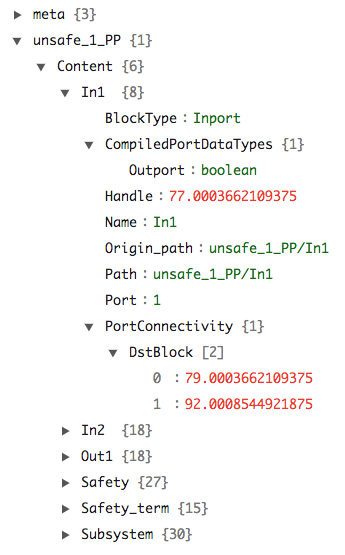
\includegraphics[scale=0.4]{figures/In1}
\end{center}  
  \caption{A JSON Representation of the CoCoSim Model}
  \label{jsoninport}
\end{figure}

\begin{figure}[h]
\begin{center}
  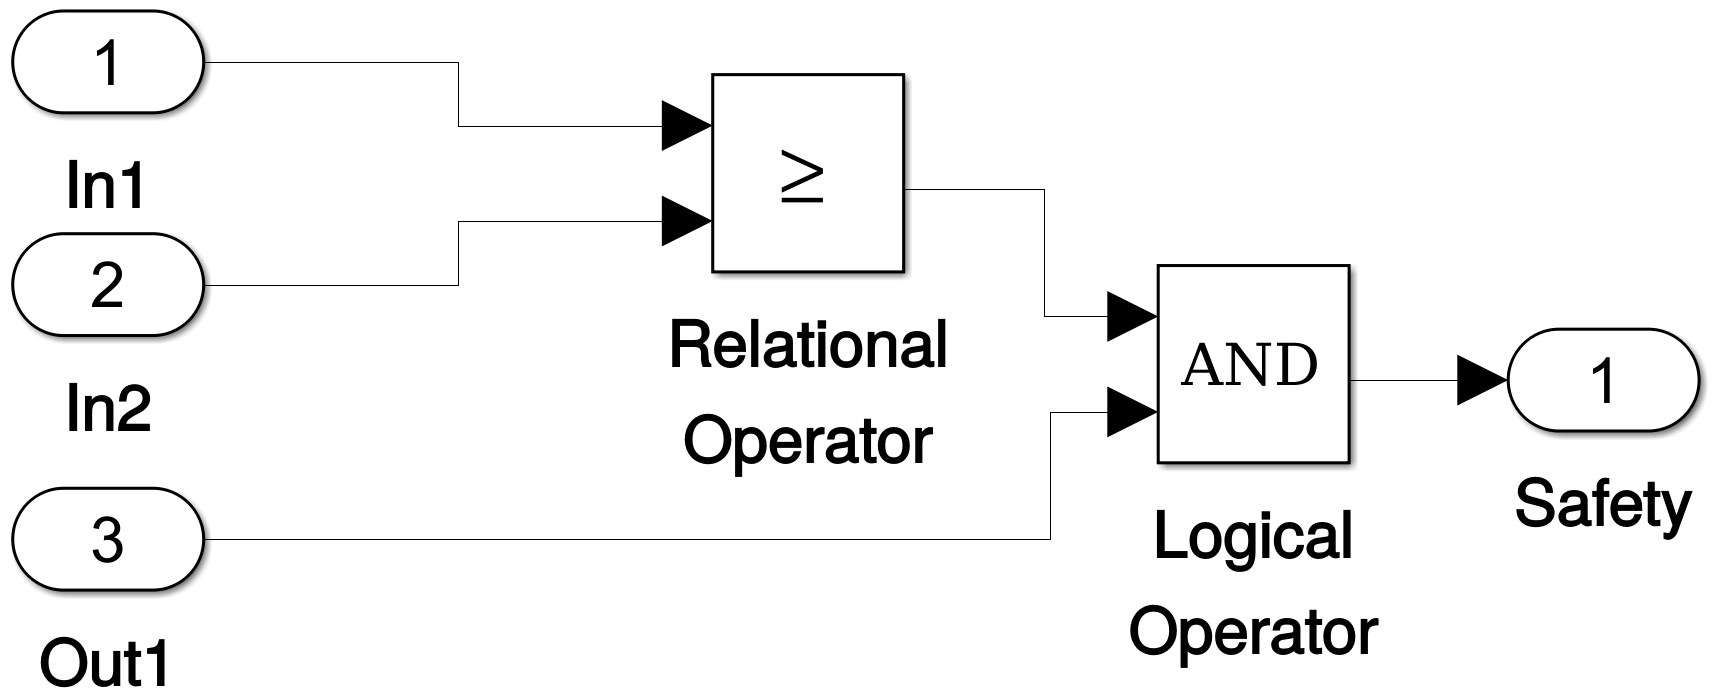
\includegraphics[scale=0.15]{figures/safety0}
\end{center}  
  \caption{A CoCoSim model of the observer block -- safety}
  \label{cocosimsafety}
\end{figure}


\begin{figure}[h]
\begin{center}
  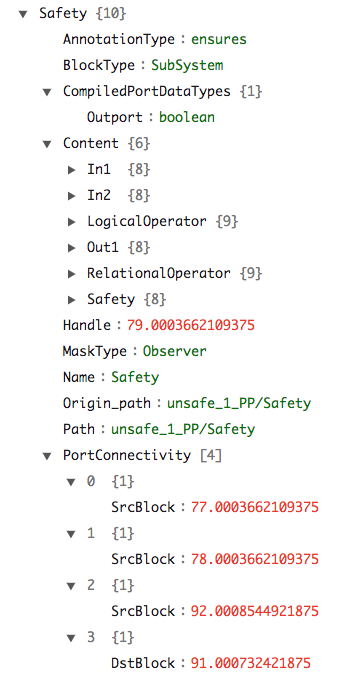
\includegraphics[scale=0.35]{figures/safety}
\end{center}  
  \caption{A JSON snippet of the observer block -- safety}
  \label{jsonsafety}
\end{figure}

\begin{figure}[h]
\begin{center}
  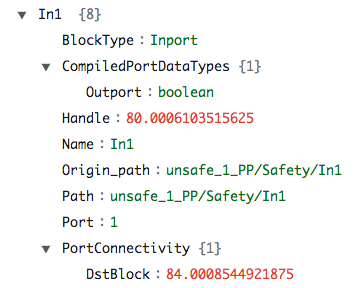
\includegraphics[scale=0.35]{figures/safety1}
    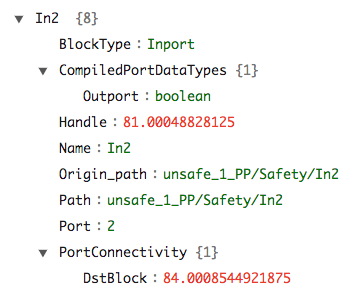
\includegraphics[scale=0.35]{figures/safety2}
  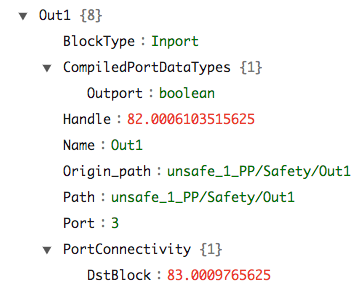
\includegraphics[scale=0.35]{figures/safety4}     
    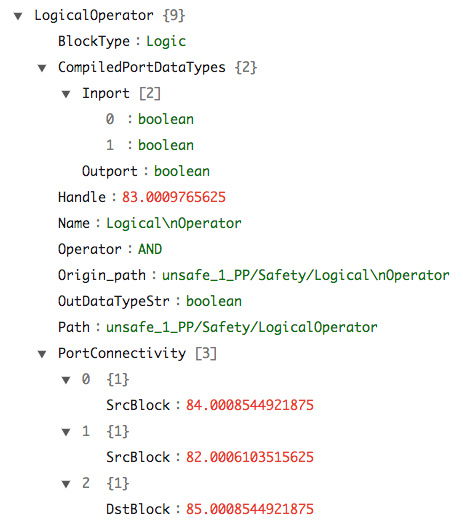
\includegraphics[scale=0.35]{figures/safety3}
    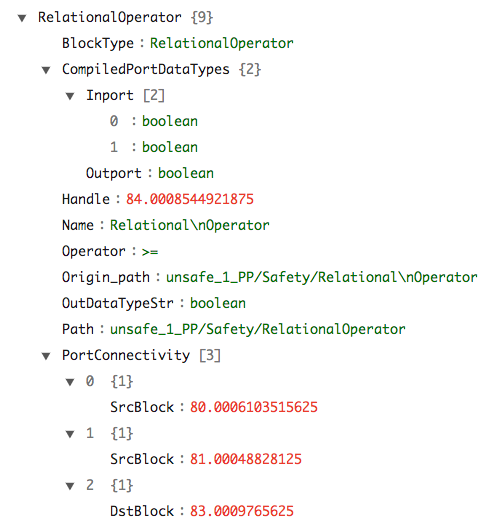
\includegraphics[scale=0.35]{figures/safety5}      
    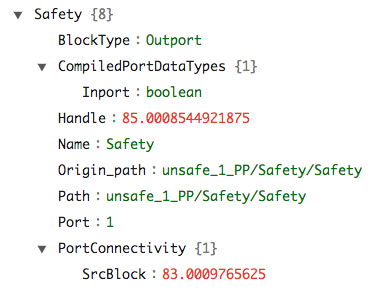
\includegraphics[scale=0.35]{figures/safety6}       
    
\end{center}  
  \caption{A JSON snippet of the body of the observer block \textsf{safety}}
  \label{jsonsafetybody}
\end{figure}

\subsection{CoCoSim Stateflow in JSON}

\begin{figure}[h]
\begin{center}
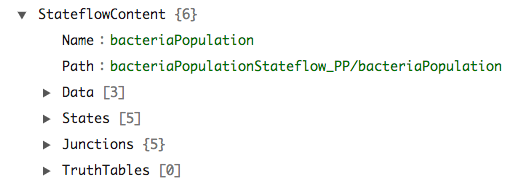
\includegraphics[scale=0.4]{figures/stateflow_json}
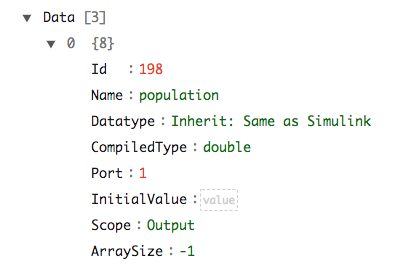
\includegraphics[scale=0.4]{figures/data}
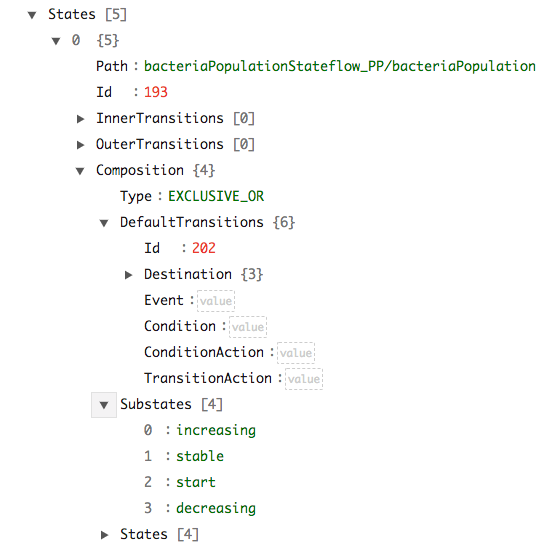
\includegraphics[scale=0.35]{figures/state}
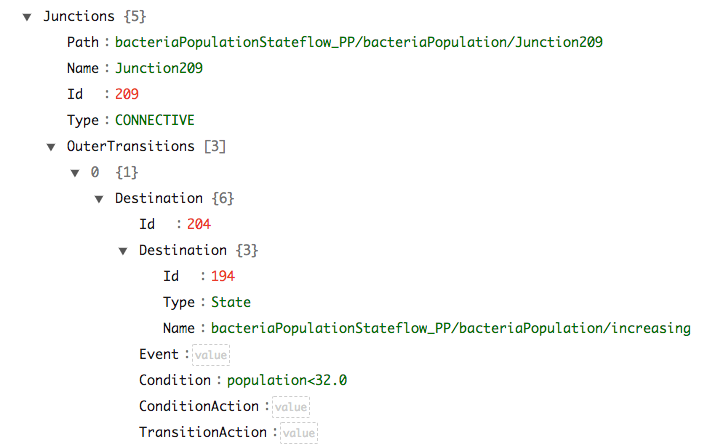
\includegraphics[scale=0.35]{figures/junction}
\end{center}  
\caption{The Stateflow definition in JSON}
\label{stateflow_json}
\end{figure}

A Stateflow is defined as the value of \textsf{StateflowContent} in JSON.
The translation supports \textsf{Data}, \textsf{States}, \textsf{Junctions}, and \textsf{Truthtables}, where each of them
is an array of items as shown in the example in Figure~\ref{stateflow_json}.
\textsf{Data} defines input, output, and local variables used in the Stateflow.
\textsf{States} defines state information and its composition such as state path, substates inside and transitions out of it, whereas \textsf{Junctions} defines transitions associated with condition, condition actions and transition actions.


\section{Mapping from Basic CoCoSim Blocks to Lustre Constructs}

\begin{figure}[h]
\begin{center}
  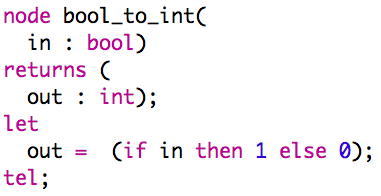
\includegraphics[scale=0.3]{figures/lus0}
  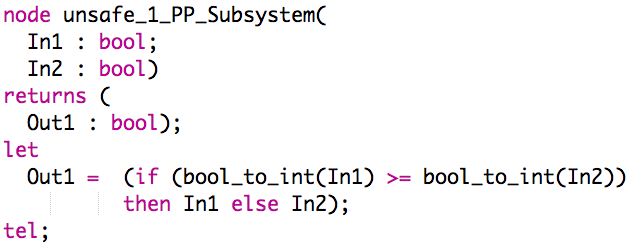
\includegraphics[scale=0.3]{figures/lus1}
  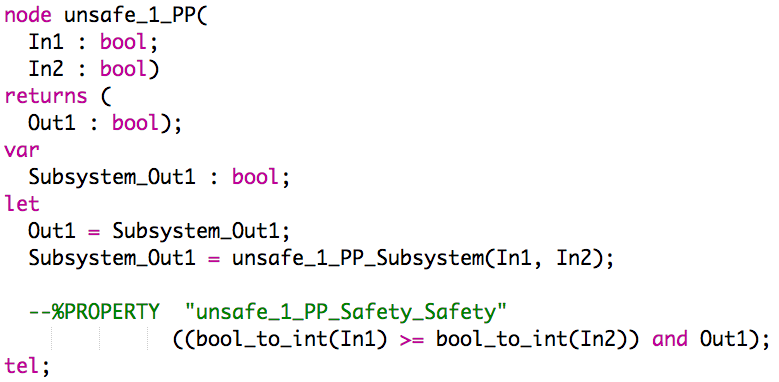
\includegraphics[scale=0.3]{figures/lus2}      
\end{center}  
  \caption{The translated Lustre programs for the CoCoSim model \textsf{unsafe\_1\_PP}}
  \label{lus}
\end{figure}

Figure~\ref{basicmapping} shows a mapping from basic CoCoSim blocks to their equivalent representations in Lustre, which is currently supported by the translator. 

\subsection{CoCoSim constructs to Lustre constructs}

\begin{figure}[t]
\centering
{
\begin{tabular}{lp{7cm}}
\hline
\textbf{CoCoSim} & \textbf{Lustre}  \\
\hline
SubSystem & 
Node
\\
Inport &
Input
\\
Outport &
Output
\\
Gain &
Multiply input by constant ($\times$)
\\

Product &
Multiply and divide scalars and nonscalars ($\times$)
\\

Abs (in) &
create library node abs
\\

AND, OR, NAND, NOR,
&
and, or, not and, not or
\\
XOR, NXOR, NOT
&
xor, not xor, not
\\
Minmax &
{Dynamically create minimum or maximum nodes}
\\

Switch &
{if ... then ... else ... }
\\

Sum &
$+$
\\

Saturate &
The Saturation block imposes upper and lower limits on an input signal ($<=, <$)
\\

RelationalOperator &
$==, <>, <, <=, >, >=$
\\

UnitDelay/Memory &
pre
\\

Vector Concatenation &
Concatenate vectors horizontally and vertically
\\

Selector &
Select elements at certain indices
\\

Demux/Mux &
Extract and output elements of vector signal/Combine input signals of same data type into vector
\\

Data Type Conversion &
Create Lustre library nodes for conversions among Boolean, Integer and Real
\\

Rounding &
Create Lustre library nodes for floor, ceiling, round and fix.  
\\

Compare To Zero/Constant  &
$==, <>, <, <=, >, >=$
\\

mod, substract, divide, negative &
mod, $\times, -, /, - $, 
\\

Constant &
constant
\\

\hline
\end{tabular}
}
\caption{A mapping from basic CocoSim blocks to Lustre constructs}
\label{basicmapping}
\end{figure}


\paragraph{Subsystem, Inport, and Outport} 
Subsystems create a hierarchical model comprising many layers. 
A subsystem is a set of blocks that you replace with a single \textsf{Subsystem} block. 
Subsystem normally consists of a set of inports and a set of outports, where outports are
defined by using inports and other blocks. 
In principle, almost all subsystems are translated into nodes in Lustre with inports being the 
inputs and outports being the outputs except for the observer subsystems and other minor blocks. 
The order of inputs and outputs are maintained during the translation. 
The hierarchical information about the model is translated into node calls.

An exception would be the observer node.
It will be inlined in the calling node as property statements instead of translating them 
as separate nodes.

\*

\indent \indent \indent \indent \textsf{-\ -\%PROPERTY ``property name" property\_expression}

\*


\noindent The \textsf{property name} is the output variable name corresponding to the property, 
and the property expression is translated by substituting the input and output variables by concrete ones.

The translation is initiated by translating the outports backwardly. 
Each outport and its connected expressions are translated into an equation, where the outport is the output of the equation 
and the right hand side of the equation is the definition of the output.
The right hand side expression is translated recursively.
Figure~\ref{lus} shows the Lustre programs translated from the CoCoSim model ``unsafe\_1\_PP".
Each expression is defined in terms of the following operators. 
We will describe the mappings of those operators in Lustre in the following paragraphs.

\paragraph{Subsystem} 
Typically, if a subsystem is within another subsystem, it will be translated as a node call.


\paragraph{Relational Operators} 
Relational operators greater than, less than, equal to, not equal to, greater 
than or equal to, and less than or equal to are translated into their counterparts 
($>, <, =, <>, >=, <=$) in Lustre.


\paragraph{Logical Operators} 
Logical operators \textsf{AND, OR, NOT} and \textsf{XOR} are translated into Lustre operators 
\textsf{and, or, not} and \textsf{xor}.
Logical operators \textsf{NAND, NOR}, and \textsf{NXOR} are represented by using Lustre 
operators \textsf{NOT} and \textsf{AND, OR, XOR}.

\paragraph{Mathematical Operators} 
Mathematical operators sum, subtract, multiply, divide and mod are translated into 
\textsf{+}, \textsf{-}, \textsf{*}, \textsf{div} and \textsf{mod} respectively.
Operator Gain is translated into \textsf{*}. 
Operator Abs is translated into a node Abs. 
Operator Minmax is translated into a node Min or Max depending on the semantics of the subsystem. 
Operator CompareToZero/Constant is translated into a Lustre expression to compare to zero or a constant. 

\paragraph{Time Operators}
Operators Memory and UnitDelay are translated into the same time operator \textsf{pre} with the 
values of First and X0 as their initial conditions respectively.
Since Memory and UnitDelay may introduce the circular dependency issue, we create local variables for the portion of expression under \textsf{pre} to break the circular dependency if any. 

\paragraph{Vector/Matrix Related Operators}
Vector Concatenation, Selector, Demux and Mux are translated into array operations in Lustre based on their semantics. 
The translation currently supports vector/matrix concatenation horizontally and vertically. 
Vector selector is represented by using access notations for array elements in Lustre, similarly for Demux and Mux. 

\paragraph{Rounding and Data Type Conversion}

Rounding blocks including \textsf{Floor, Ceil, Round}, and \textsf{Fix} are translated as Lustre Nodes. 
Since Kind 2 supports conversion between Real and Integer by using two keywords \textsf{"real"} and \textsf{"int"},
we use them to create a node to encode the operator \textsf{floor} as $floor = \textsf{real} (\textsf{int}$ $x)$, where $x$ and $floor$ are both real numbers and $floor$ is the result of applying operator \textsf{floor} on $x$. 
And the \textsf{ceil} block is encoded in terms of \textsf{floor} as $ceil = -\textsf{floor}(-x)$.
Round block is translated to a node \textsf{round} with its body equation defined as $round = \textsf{if}$ $x >= 0.0$ $\textsf{then}$ $\textsf{ceil}(\textsf{abs}(x))$ \textsf{else} $-\textsf{ceil}(\textsf{abs}(x))$, where \textsf{abs} is a Lustre node to compute the absolute value of the input.
Fix block is translated to a node \textsf{fix} with its body equation defined as $fix = \textsf{if}$ $x >= 0.0$ $\textsf{then}$ $\textsf{floor}(\textsf{abs}(x))$ \textsf{else} $-\textsf{floor}(\textsf{abs}(x))$.
Data Type Conversion block is translated either using keywords \textsf{real} and \textsf{int} or Lustre library nodes. 
For data types conversions between integer and real numbers, we use keywords \textsf{real} and \textsf{int} respectively. 
For data types conversions between \textsf{bool} and \textsf{integer(real)}, we use library nodes \textsf{bool\_to\_int, bool\_to\_real, int\_to\_bool} and \textsf{real\_to\_bool} respectively, where \textsf{bool\_to\_int} and \textsf{bool\_to\_real} are defined as $output =$ \textsf{if} $input$ \textsf{then} $1(1.0)$ \textsf{else} $0(0.0)$
, and \textsf{int\_to\_bool} and \textsf{real\_to\_bool} are defined as $output =$ \textsf{if} $input = 0(0.0)$ \textsf{then} $true$ \textsf{else} $false$.


\begin{figure}[t]
\[
\begin{array}{l@{\qquad}llll}
 \text{constant} & c & := & 
true \mid false
 \\[0ex]
 \text{number} & n & := & 
 1 \cdots 9 (.1 \cdots 9)
 \\[0ex]
  \text{literal} & v & := & 
u n \mid n \mid c
 \\[0ex]
\text{unary expression} & e & := & 
-\ e \mid \sim e \mid \sim b \mid v
 \\[0ex]
 \text{binary expression} & b & := & 
e_1\ (>, <, >=, <=, ==, \sim=)\ e_2 
 \\[0ex]
\end{array}       
\]
\caption{The syntax for the conditional expresions}
\label{fig:grammar}
\end{figure}

\paragraph{Conditional Operators}
Operator SwitchCase is translated into \textsf{if $\cdots$ then $\cdots$ else if $\cdots$ then $\cdots$ }. 
For the IF operator, the conditional expressions are translated separately using the
expression parser \emph{ParBoiled} as the conditional expressions are in the string format. 
The expressions are defined by the syntax in Figure~\ref{fig:grammar}.

When parsing the expressions, the expression will be constructed as an abstract syntax tree. 
As we traverse the abstract syntax tree, the variables will be substituted by the concrete expressions corresponding to them.

\subsection{Types}

Types in CoCoSim models are not strictly defined. 
They can be mixed compared, i.e., an integer can compare to a Boolean.
However, Lustre language is a strictly typed language.
To be better handle types in CoCoSim models, we define six auxiliary functions
for converting typed expressions.
They are \textsf{bool\_to\_int, bool\_to\_real, int\_to\_bool, 
real\_to\_bool, real\_to\_int} and \textsf{int\_to\_real}. 

While translating expressions comparisons, if two different typed expressions, their types will be lifted to the highest type.
If Boolean typed expressions are compared, they will be converted to integer and compare.
For example, in the ``unsafe\_1\_PP" model, since the inputs In1 and In2 are Boolean types but we are comparing them, we need to lift their types to integer by wrapping them with \textsf{bool\_to\_int} and do the comparison afterwards. 
If an expression is typed with Integer or Real and it is used as Boolean in the model,  it will be lowered 
to a Boolean by calling the function \textsf{int\_to\_bool} or \textsf{real\_to\_bool}.
 

\subsection{Translation of CoCoSim contracts}

\begin{figure}[h]
\begin{center}
  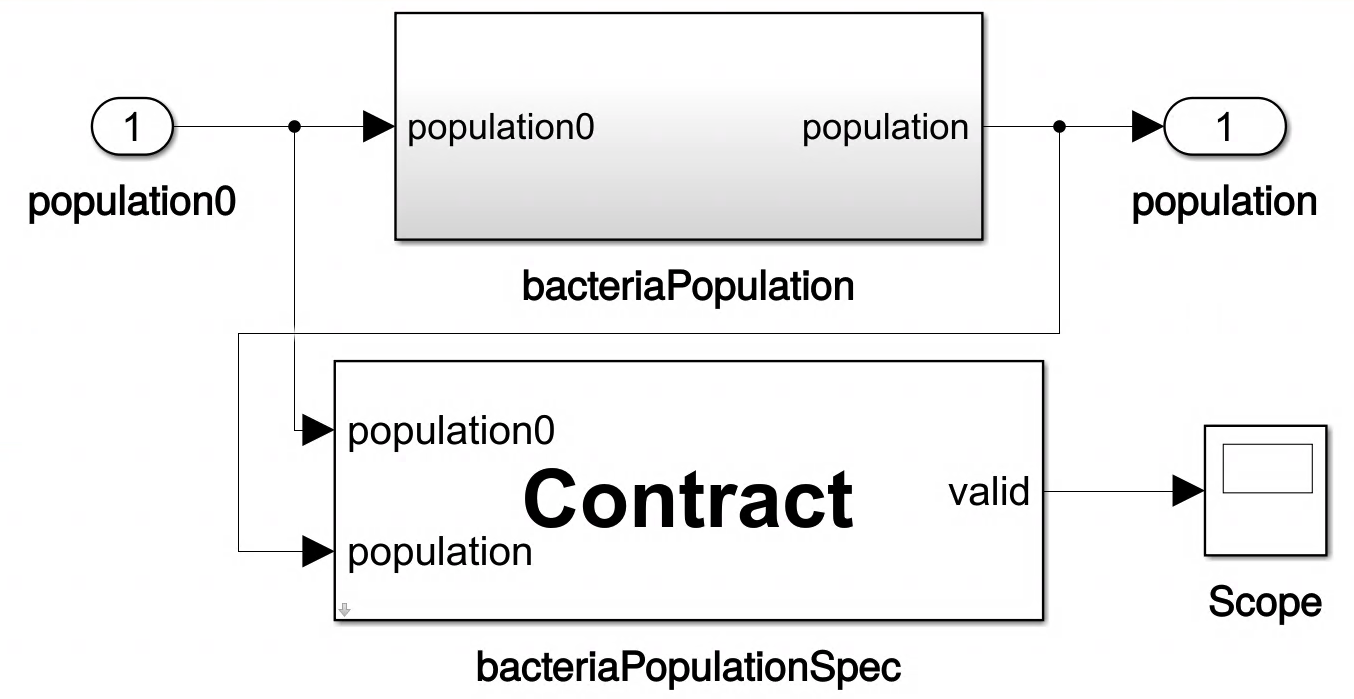
\includegraphics[scale=0.2]{figures/contract}    
\end{center}  
  \caption{A CoCoSim model using contracts}
  \label{contractmodel}
\end{figure}


The Kind 2 contracts are introduced as additional features for modeling CoCoSim models.
They are encapsulated in \textsf{Subsystem} blocks and are accessible by using customized 
blocks.
To distinguish different contract blocks, we use the \textsf{``ContractBlockType"} in JSON to indicate whether a block 
is an \textsf{assume}, \textsf{guarantee}, \textsf{mode}, \textsf{requires}, or \textsf{ensures} block.
The contract block always returns a Boolean variable \textsf{valid}.
The translation ignores the output variable \textsf{valid} and construct the signature 
of the contract by identifying with the signature of the calling node.
The translation of expressions of contracts is the same as translating expressions in the subsystem blocks.

\begin{figure}[h]
\begin{center}
  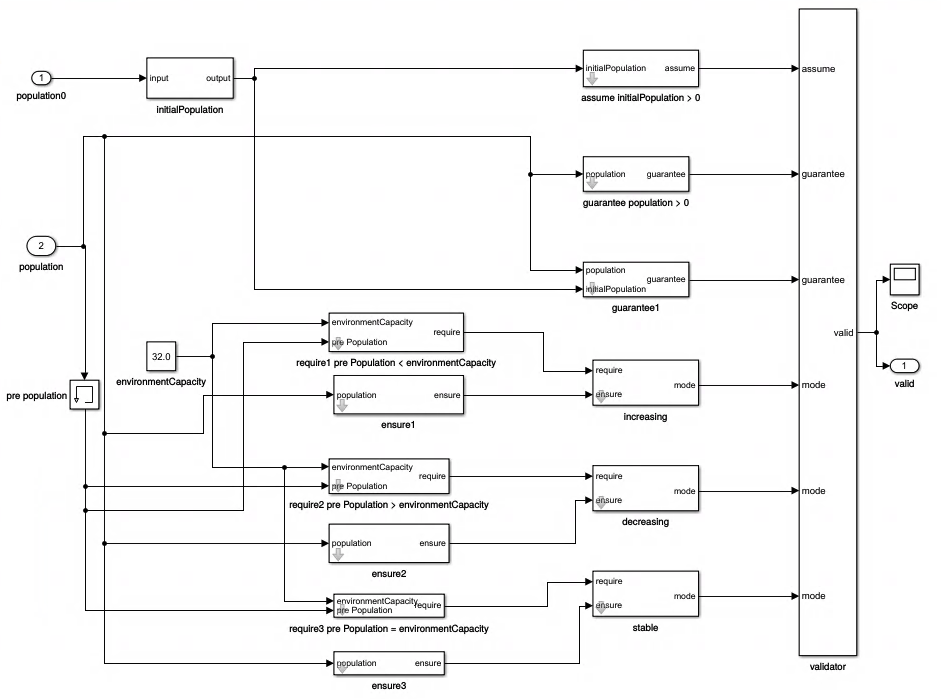
\includegraphics[scale=0.5]{figures/contract1}    
\end{center}  
  \caption{The contract body definition}
  \label{contractdef}
\end{figure}

\begin{figure}[h]
\begin{center}
  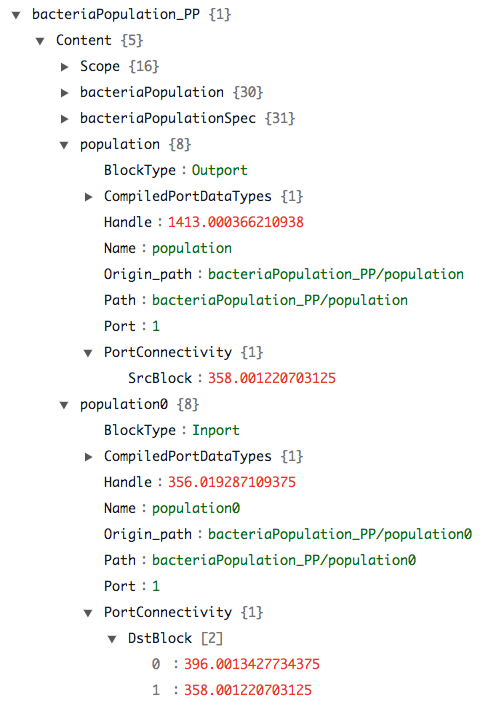
\includegraphics[scale=0.45]{figures/jsoncontract}    
\end{center}  
  \caption{The overview of CoCoSim model bacterialPopulation in JSON}
  \label{jsoncontract}
\end{figure}

\begin{figure}[h]
\begin{center}
  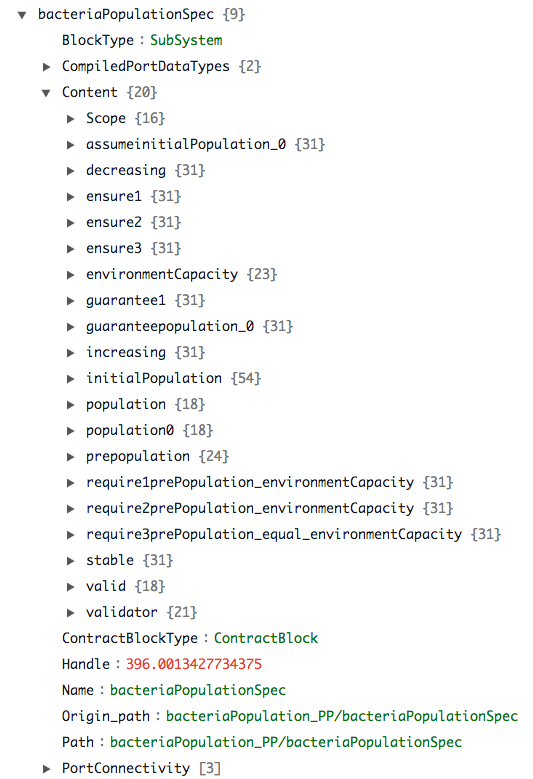
\includegraphics[scale=0.4]{figures/jsoncontractdef}    
\end{center}  
  \caption{The contract of bacterialPopulation in JSON}
  \label{jsoncontractdef}
\end{figure}

\begin{figure}[h]
\begin{center}
  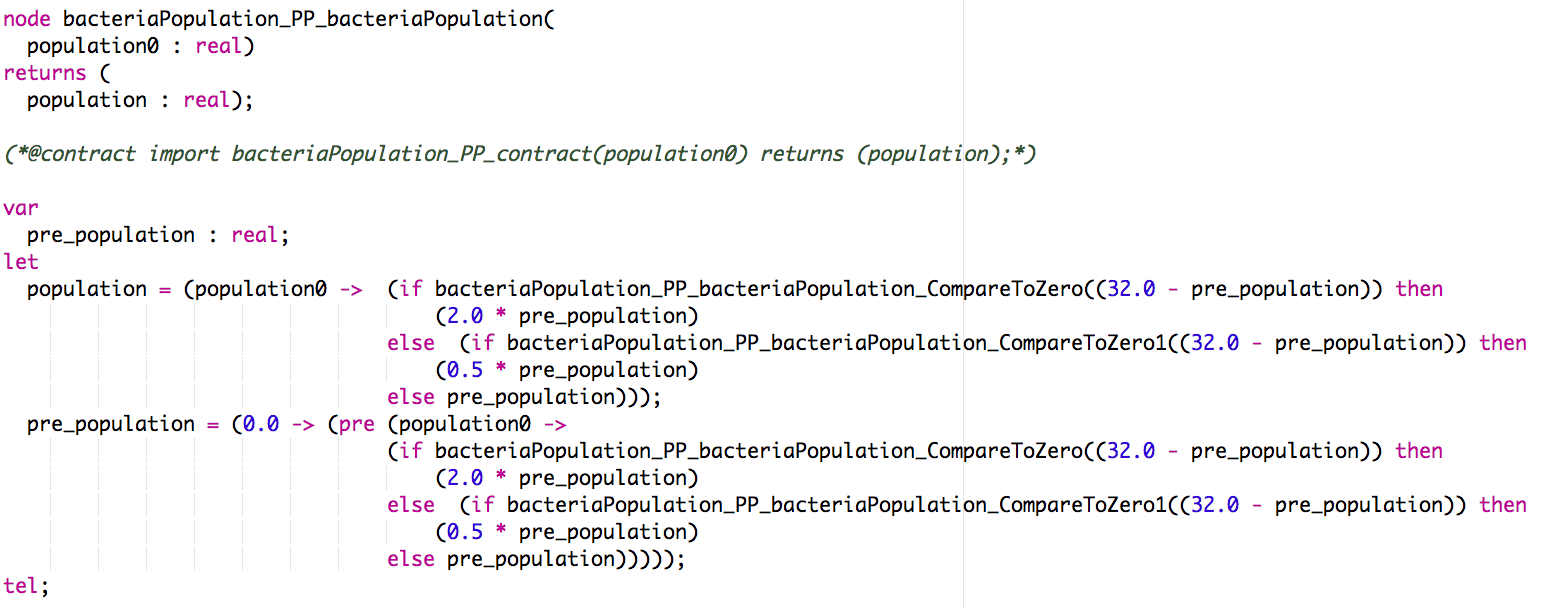
\includegraphics[scale=0.3]{figures/lusnodecon}    
\end{center}  
  \caption{The bacterialPopulation node with contract in Lustre}
  \label{lusnodecon}
\end{figure}

\begin{figure}[h]
\begin{center}
  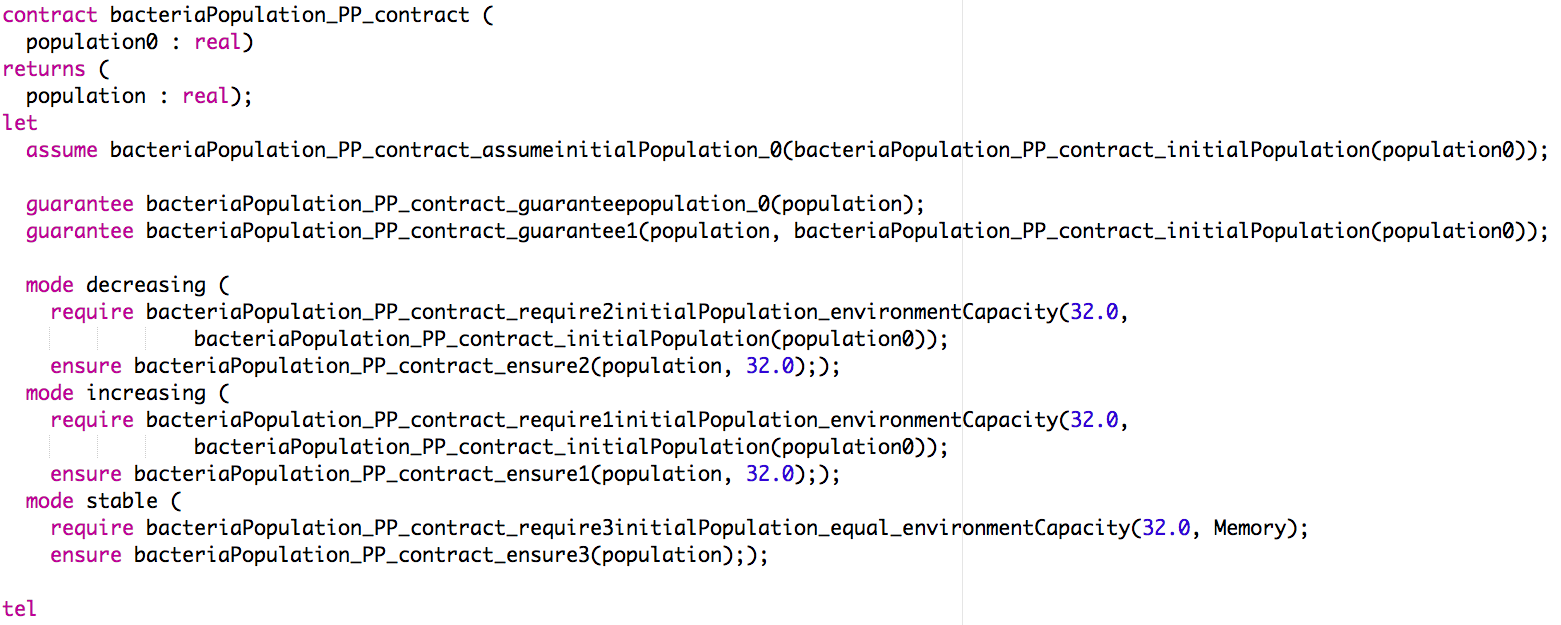
\includegraphics[scale=0.3]{figures/luscon}    
\end{center}  
  \caption{The bacterialPopulation contract in Lustre}
  \label{luscon}
\end{figure}

Figure~\ref{contractmodel} shows a CoCoSim model ``bacterialPopulation" using contracts. 
And the contract body definition is shown in Figure~\ref{contractdef}, where it has one \textsf{assume}, two \textsf{guarantees}, and three \textsf{mode} connecting to the \textsf{validator} block. 
The \textsf{validator} block always has an outport \textsf{valid}. 
Figure~\ref{jsoncontract} and Figure~\ref{jsoncontractdef} are the overview of CoCoSim model \textsf{``bacterialPopulation"} and its contract definition in JSON respectively. 
The Lustre programs translated from the JSON model of the bacterialPopulation are shown Figure~\ref{lusnodecon}~\ref{luscon}.

\subsection{Translation of Stateflow Charts}

\subsubsection{Stateflow}
\begin{figure}[h]
\begin{center}
  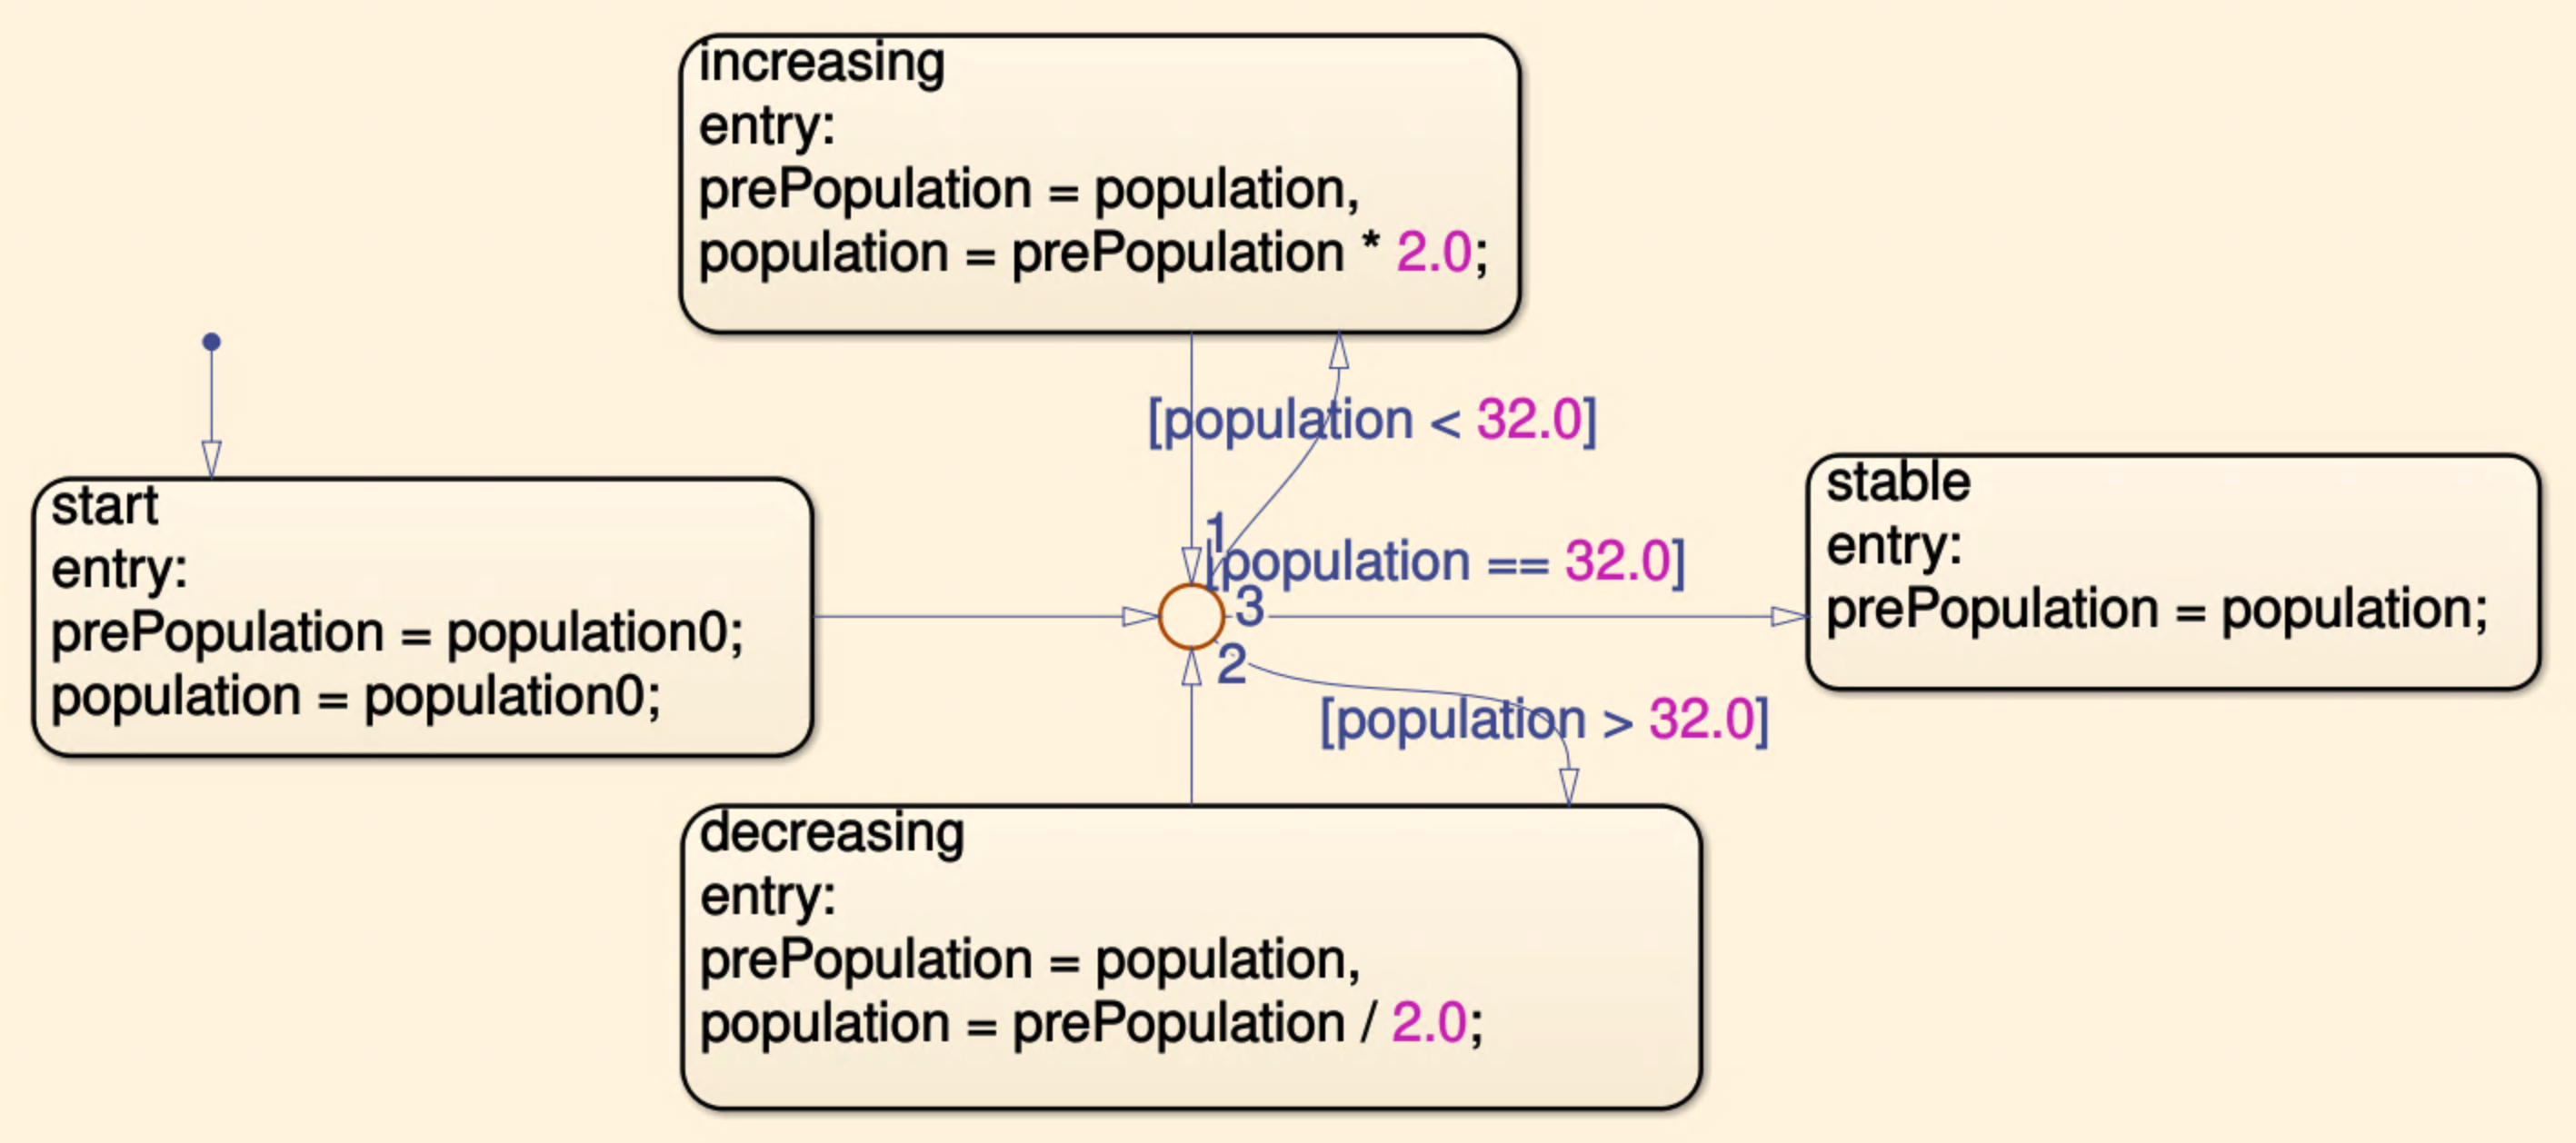
\includegraphics[scale=0.2]{figures/sf}    
\end{center}  
  \caption{A stateflow example}
  \label{sf}
\end{figure}

Stateflow is an extension of Simulink for modeling and simulating decision logic based on state machines and flow charts. 
Stateflow including state transition diagrams, flow charts, state transition tables, and truth tables, allows to model how your system reacts to events, conditions, and external inputs.
Stateflow can also be used to model state machines and its behaviors. 
Figure~\ref{sf} shows a stateflow example, which has 4 states start, decreasing, increasing, and stable and a junction. 
Each state transits to the same junction without any condition. 
The junction transits to decrease, stable, or increase state depending on the condition, whether \textsf{population} is greater than, equal to or less than 32.0. 
Stateflow is translated into Lustre automaton based on its semantics. 

\subsubsection{Translation of States}
Staeflow has two types of states: exclusive and parallel. 
State can be nested in another state.
Each state has nine different actions i.e., Entry, During, Exit, Bind, On, OnAfter, OnBefore, OnAt, and OnEvery. 
Among those, the translation currently only supports Entry, During and Exit actions. 
Stateflow State is translated into an automaton state in Lustre with its during actions as its body equations.
An initialization state is created with the Entry actions of the first state of the system as its body equations. 
A center point state is created as the initial state to control the transitions. 
A transition in Stateflow charts is encoded as a strong transition in Lustre ``\textsf{unless} condExpr \textsf{restart} stateName".

We create a state id for each original state of the system with 0 being the id for the initialization state.
We currently support exclusive states with no nested states.
For each simple transition from a state \textsf{src} to another state \textsf{dest} with a condition \textsf{condExpr}, condition actions \textsf{condActions} and transition actions \textsf{transitActions}, we create a Lustre automaton state  \textsf{src\_to\_dest} with condition actions \textsf{condActions}, transition actions \textsf{transitActions}, the Exit actions of \textsf{src} and the Entry actions of \textsf{dest} being its body equations.
At each Lustre automaton state, we set the next active state id to the id of the destination state.
For example, at the state \textsf{src\_to\_dest}, we would set the next active state id to the id of the \textsf{dest} state.
After executing all the actions, each state will go back to the center point state via weak transition ``\textsf{unless} true \textsf{restart} center\_point\_state".


The execution order of transitions in the Stateflow is maintained in the strong transitions of the initial Lustre automaton state by following the 12 o'clock rule in Stateflow chart.
The transition at 12 o'clock is evaluated first and the rest is evaluated from top to bottom and from left to right. 
Therefore, we put the transition condition of the transition at 12 o'clock at the top and the rest is listed following from top to bottom and from left to right. 

\subsubsection{Translation of Junctions}

\begin{figure}[h]
\begin{center}
  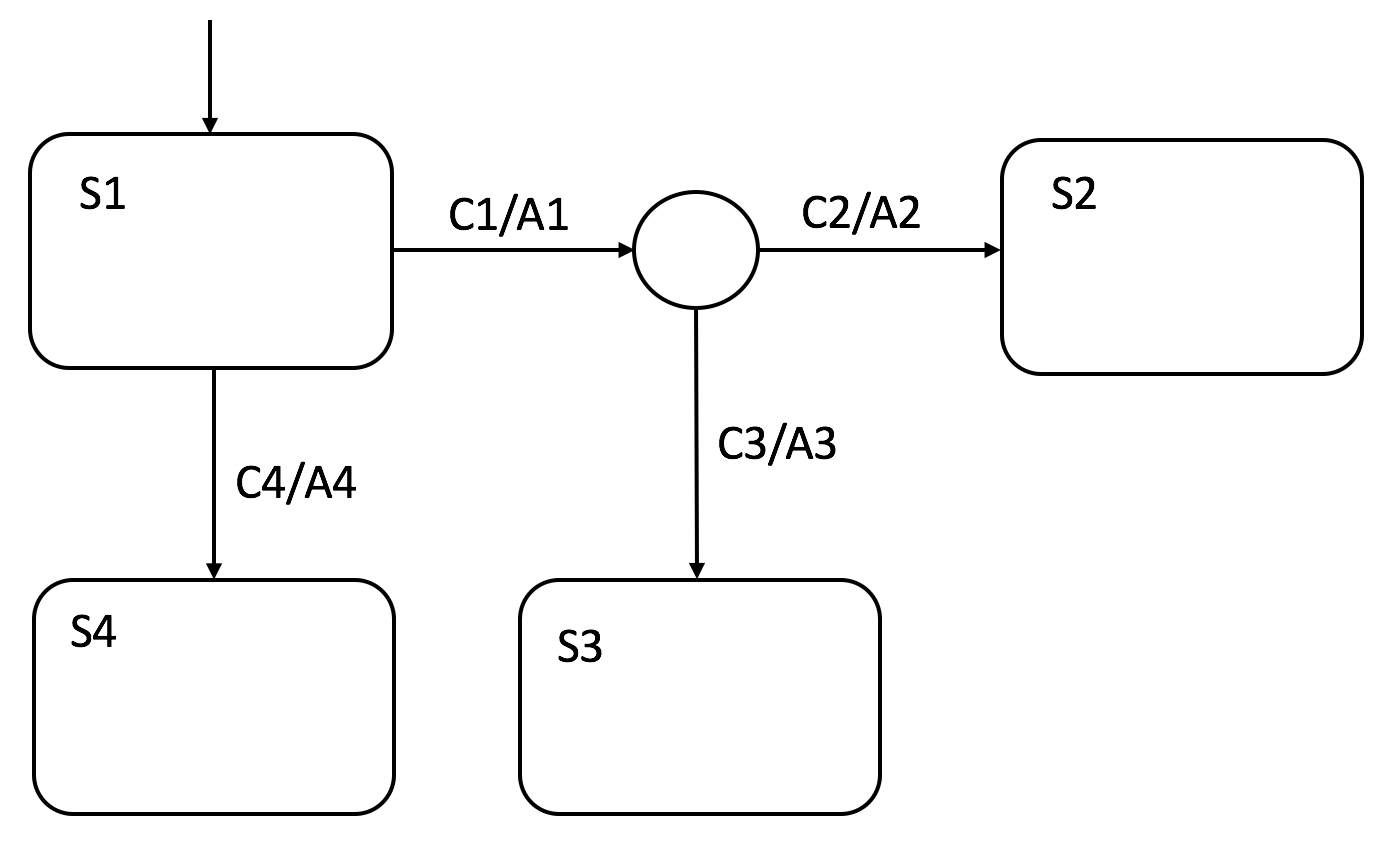
\includegraphics[scale=0.18]{figures/sf1} 
    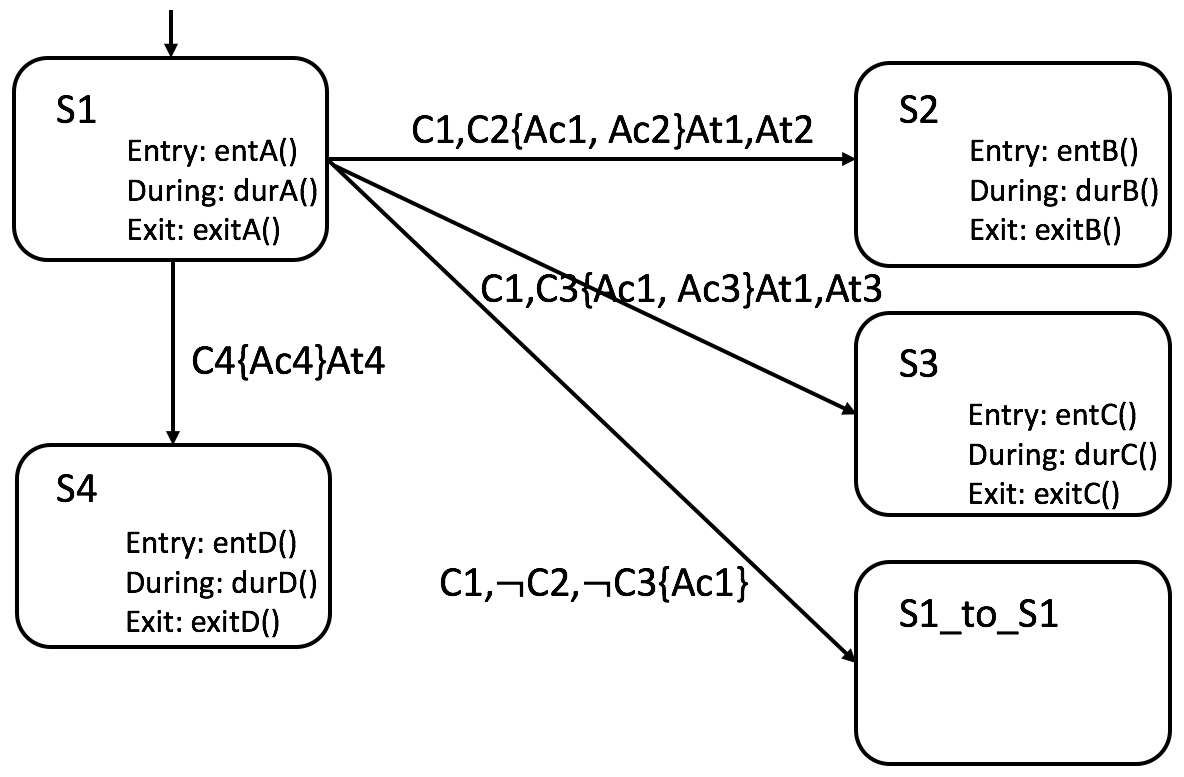
\includegraphics[scale=0.15]{figures/sf2}    
\end{center}  
  \caption{Conversion from stateflow chart with junctions to another one without junctions}
  \label{sf1}
\end{figure}

\begin{figure}[h]
\begin{center}
  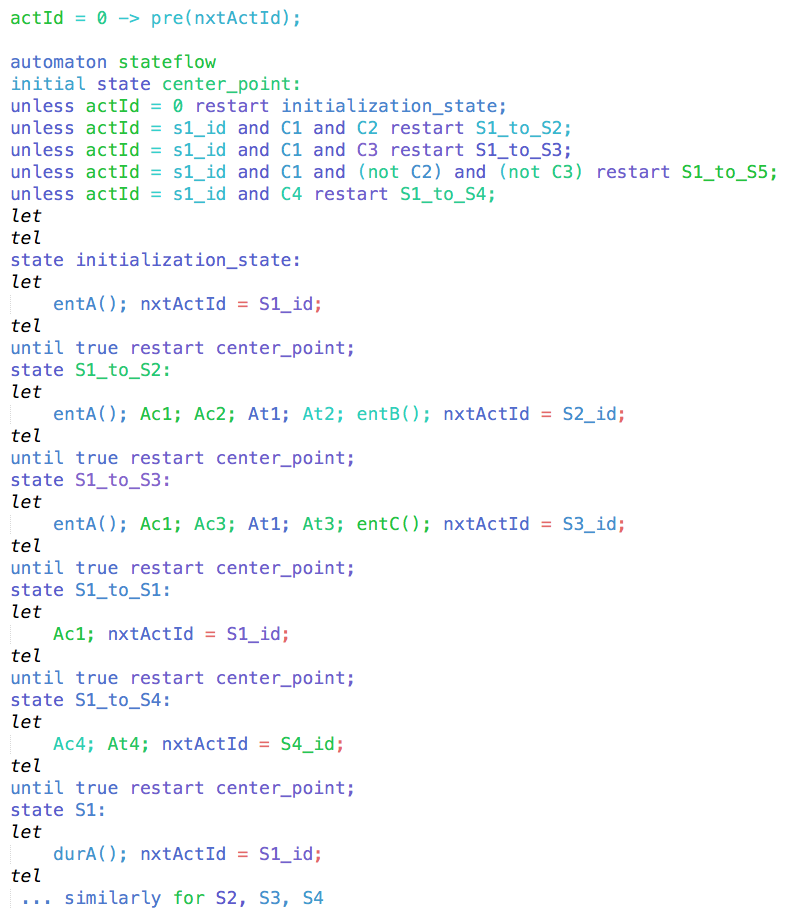
\includegraphics[scale=0.3]{figures/automaton} 
\end{center}  
  \caption{The Lustre automaton for the stateflow in Figure \ref{sf1}}
  \label{automaton}
\end{figure}

A junction is a decision point for transitions. 
Junctions are compressed to simple transitions to states based on its semantics. 
A simple transition is defined as a transition from a state to another state based on some condition. 
Figure~\ref{sf1} shows a conversion from a stateflow chart with junctions to an equivalent one without junctions.
Compression of junctions follows the evaluation rule of junctions in stateflow charts.
Consider the example in Figure~\ref{sf1}, there are 4 states and 1 junction in the original stateflow chart on the left, where S1 is the start state.
At the beginning of the system clock tick, the system starts evaluating C1 and C2, if C1 and C2 are both valid, it execute S1's exit actions, Ac1, Ac2, At1, At2 and entB() and set the next active state id to the id of S2. 
In this case, we compress together conditions C1 and C2 on the junction, and create a new state \textsf{S1\_exit\_to\_S2\_entry} with S1's exit actions, Ac1, Ac2, At1, At2 and entB() being its body equations. 
Similarly, if C2 is valid and C3 is valid, the system execute S1's exit actions, Ac1, Ac3, At1, At3 and entC() and set the next active state id to the id of S3, and we create a new state for the transition from S1 to S3.
If C2 and C3 are both invalid and C1 is valid, the system execute Ac1 and set the next active state id to the id of S1.
If C1 is invalid and C4 is valid, the system execute S1's exit actions, Ac4, At4, and entD().  
Otherwise, it will stay in S1 and execute S1's During actions. 
Figure~\ref{automaton} shows the Lustre automaton for the stateflow in Figure~\ref{sf1}.


\subsection{Mapping Information}

The translation yields a JSON file for mapping purpose between the input Simulink model and the output Lustre program. 
For each subsystem block except for the observer block in Simulink, the translation generates its origin path in the Simulink model and its node name in Lustre as the values for \textsf{OriginPath} and \textsf{NodeName} in JSON respectively.
And for each inport and outport of a subsystem block, it also generates its variable name in the Lustre program as the value for \textsf{VariableName} additionally.
For each contract block, the translation produces its \textsf{OriginPath} in the Simulink model and its contract name \textsf{ContractName} in Lustre with inports and outports names as \textsf{VariableName} in JSON.
The translation generates a property name and index for each assumption and guarantee as the values of \textsf{PropertyName} and \textsf{Index} in addition to its \textsf{OriginPath} and \textsf{ContractName}.
For each require and ensure in a mode of a contract, it produces its origin path, contract name, require/ensure name, mode name and index as the values of 
\textsf{OriginPath}, \textsf{ContractName}, \textsf{PropertyName}, \textsf{Index} and \textsf{ModeName}.

\section{The Translation Algorithms}

We describe here the translation algorithms for the JSON model in Figure~\ref{mainalgo}~\ref{mainalgo1}~\ref{translateblock}~\ref{translatenode}~\ref{translatecontract}.
Figure~\ref{mainalgo} is the entry point of the translation algorithm, where it takes the root node of the JSON file as input and returns a Lustre program for it.
The algorithm first recursively collect all subsystem blocks in the root node, and then translate each of them by calling the function \textsf{translateSubsystem}. 
If the node is a contract, it will invoke \textsf{translateForContract}, 
otherwise, it will call \textsf{translateForLusNode}.


\begin{figure}
\begin{algorithmic}
\Function{\textbf{translate}}{\textbf{Node} rootNode}
\\
\Return{(\textbf{LustreProgram} P)}
\State \textbf{let} subsystems = \{S $\mid$ S is a subsystem block $\land$ S $\in$ rootNode.fields\} \textbf{in}
\State \textbf{for} subsystem : subsystems
\State {\ \ \ \ } \textbf{let} \textbf{LustreAst} ast = \textbf{translateSubsystem}(subsystem) \textbf{in}
\State {\ \ \ \ } \textbf{if}  ast \textbf{instanceof} LustreNode \textbf{then}
\State {\ \ \ \ \ \ \ \ } P.\textbf{addNode}(ast)
\State {\ \ \ \ } \textbf{else}
\State {\ \ \ \ \ \ \ \ } P.\textbf{addContract}(ast)
\EndFunction
\end{algorithmic}
\label{mainalgo}
\caption{The entry point for the translation algorithm}
\end{figure}

\begin{figure}
\begin{algorithmic}
\Function{\textbf{translateSubsystem}}{\textbf{Node} subsystem}
\\
\Return{(\textbf{LustreAst} ast)}

\State \textbf{let} inputs = \{\} \textbf{in}
\State \textbf{let} props = \{\} \textbf{in}
\State \textbf{let} outputs = \{\} \textbf{in}
\State \textbf{let} contract = \{\} \textbf{in}
\State \textbf{let} hdlToBlk = \{\} \textbf{in}
\State \textbf{let} blkToSrcHdls = \{subsystem $\mapsto$ subsystem.\textbf{getSrcHdls}()\} \textbf{in}
\State \textbf{let} blkToDstHdls = \{subsystem $\mapsto$ subsystem.\textbf{getDstHdls}()\} \textbf{in}
\State \textbf{for} cntBlk : subsystem.\textbf{contentFields}()
\State {\ \ \ \ }  blkToSrcHdls $\leftarrow$ \{cntBlk $\mapsto$ cntBlk.\textbf{getSrcHdls}()\};
\State {\ \ \ \ }  blkToDstHdls $\leftarrow$ \{cntBlk $\mapsto$ cntBlk.\textbf{getDstHdls}()\};
\State {\ \ \ \ } hdlToBlk $\leftarrow$ \{cntBlk.\textbf{getHdl}() $\mapsto$ cntBlk\};
\State {\ \ \ \ } \textbf{match}  cntBlk.\textbf{getBlkType}() \textbf{with}
\State {\ \ \ \ } $\mid$ PROP $\rightarrow$ props $\leftarrow$ cntBlk;
\State {\ \ \ \ } $\mid$ INPORT $\rightarrow$ inputs $\leftarrow$ \{\textbf{LustreVar}(cntBlk), contBlk\}; 
\State {\ \ \ \ } $\mid$ OUTPORT $\rightarrow$ outputs $\leftarrow$ \{\textbf{LustreVar}(cntBlk), contBlk\};
\State {\ \ \ \ } $\mid$ CONTRACT $\rightarrow$ contracts $\leftarrow$ cntBlk;
\State {\ \ \ \ } $\mid$ VALIDATOR $\rightarrow$ validator $\leftarrow$ contBlk;
\State \textbf{if} subsystem.\textbf{isContract}() \textbf{then}
\State {\ \ \ \ } \textbf{translateForContract}(subsystem, validator, inputs, outputs, hdlToBlk, 
\State {\ \ \ \ \ \ \ \ \ \ \ \ \ \ \ \ \ \ \ \ \ \ \ \ \ \ \ \ \ \ \ \ \ \ \ \ } blkToSrcHdls, blkToDstHdls);
\State \textbf{else}
\State {\ \ \ \ } \textbf{translateForLusNode}(subsystem, inputs, outputs, props, contracts, hdlToBlk,
\State {\ \ \ \ \ \ \ \ \ \ \ \ \ \ \ \ \ \ \ \ \ \ \ \ \ \ \ \ \ \ \ \ \ \ \ \ } blkToSrcHdls, blkToDstHdls);
\EndFunction
\end{algorithmic}
\label{mainalgo1}
\caption{The translation algorithm}
\end{figure}


\begin{figure}
\begin{algorithmic}
\Function{\textbf{translateForLusNode}}{\textbf{Node} subsystem, \textbf{Map} inputs, \textbf{Map} outputs, \textbf{List} props, \textbf{List} contracts, \textbf{Map} hdlToBlk, \textbf{Map} blkToSrcHdls, \textbf{Map} blkToDstHdls}
\\
\Return{(\textbf{LustreAst} ast)}
\State \textbf{let} equations = \{\} \textbf{in}
\State \textbf{for} (var, outputBlk) : outputs
\State {\ \ \ \ } equations $\leftarrow$ \textbf{LusEquation}(var, \textbf{translateBlock}(outputBlk, \State {\ \ \ \ \ \ \ \ \ \ \ \ \ \ \ \ \ \ \ \ \ \ \ \ \ \ \ \ \ \ \ \ \ \ \ \ \ \ \ \ \ \ \ \ \ \ \ \ } hdlToBlk, blkToSrcHdls, blkToDstHdls));
\State \textbf{LustreNode}(inputs, outputs, props, contracts, equations);
\EndFunction
\end{algorithmic}
\label{translatenode}
\caption{The algorithm for translating the subsystem node to Lustre node}
\end{figure}


\begin{figure}
\begin{algorithmic}
\Function{\textbf{translateForLusContract}}{\textbf{JsonNode} contract, \textbf{JsonNode} validator, \textbf{Map} inputs, \textbf{Map} outputs, \textbf{List} props, \textbf{List} contracts, \textbf{Map} hdlToBlk, \textbf{Map} blkToSrcHdls, \textbf{Map} blkToDstHdls}
\\
\Return{(\textbf{LustreAst} ast)}
\State \textbf{for} srcHdl : blkToSrcHdls.\textbf{get}(validatorBlk)
\State {\ \ \ \ } \textbf{let} assumptions = \{\} \textbf{in}
\State {\ \ \ \ } \textbf{let} guarantees = \{\} \textbf{in}
\State {\ \ \ \ } \textbf{let} modeToRequires = \{\} \textbf{in}
\State {\ \ \ \ } \textbf{let} modeToEnsures = \{\} \textbf{in}
\State {\ \ \ \ } \textbf{let} srcBlk = hdlToBlk.\textbf{get}(srcHdl) \textbf{in}
\State {\ \ \ \ } \textbf{match} srcBlk \textbf{with}
\State {\ \ \ \ } $\mid$ \textbf{ASSUME} $\rightarrow$ assumptions $\leftarrow$ \textbf{translateBlock}(srcBlk, hdlToBlk, blkToSrcHdls, blkToDstHdls);
\State {\ \ \ \ } $\mid$ \textbf{GUARANTEE} $\rightarrow$ guarantees $\leftarrow$ \textbf{translateBlock}(srcBlk, hdlToBlk, blkToSrcHdls, 
\State {\ \ \ \ \ \ \ \ \ \ \ \ \ \ \ \ \ \ \ \ \ \ \ \ \ \ \ \ \ \ \ \ \ \ \ \ \ \ \ \ \ \ \ \ \ \ \ \ \ \ \ \ \ \ \ \ \ \ \ \ \ \ \ \ \ \ \ \ \ \ \ \ \ \ \ \ \ \ \ \ \ \ \ \ \  } blkToDstHdls);
\State {\ \ \ \ } $\mid$ \textbf{MODE} $\rightarrow$ \textbf{let} modeName = \textbf{getModeName}(srcBlk) \textbf{in}
\State {\ \ \ \ \ \ \ \ \ \ \ \ \ \ \ \ \ \ \ \ \ \ } \textbf{let} modeName = \textbf{getModeName}(srcBlk) \textbf{in}
\State {\ \ \ \ \ \ \ \ \ \ \ \ \ \ \ \ \ \ \ \ \ \ } \textbf{let} requires = \{\} \textbf{in}
\State {\ \ \ \ \ \ \ \ \ \ \ \ \ \ \ \ \ \ \ \ \ \ } \textbf{let} ensures = \{\} \textbf{in}
\State {\ \ \ \ \ \ \ \ \ \ \ \ \ \ \ \ \ \ \ \ \ \ } \textbf{for} modeInHdl : blkToSrcHdls.\textbf{get}(srcBlk) \textbf{in} 
\State {\ \ \ \ \ \ \ \ \ \ \ \ \ \ \ \ \ \ \ \ \ \ \ \ \ \ } \textbf{let} modeInBlk = hdlToBlk.\textbf{get}(modelInHdl) \textbf{in} 
\State {\ \ \ \ \ \ \ \ \ \ \ \ \ \ \ \ \ \ \ \ \ \ \ \ \ \ } \textbf{match} modeInBlk \textbf{with}
\State {\ \ \ \ \ \ \ \ \ \ \ \ \ \ \ \ \ \ \ \ \ \ \ \ \ \ \ \ \ \ } $\mid$ \textbf{REQUIRE} $\rightarrow$ requires $\leftarrow$ \textbf{translateBlock}(modeInBlk, hdlToBlk, blkToSrcHdls, 
\State {\ \ \ \ \ \ \ \ \ \ \ \ \ \ \ \ \ \ \ \ \ \ \ \ \ \ \ \ \ \ \ \ \ \ \ \ \ \ \ \ \ \ \ \ \ \ \ \ \ \ \ \ \ \ \ \ \ \ \ \ \ \ \ \ \ \ \ \ \ \ \ \ \ \ \ \ \ \ \ \ \ \ \ \ \ \ \ \ } blkToDstHdls);
\State {\ \ \ \ \ \ \ \ \ \ \ \ \ \ \ \ \ \ \ \ \ \ \ \ \ \ } $\mid$ \textbf{ENSURES} $\rightarrow$ ensure $\leftarrow$ \textbf{translateBlock}(modeInBlk, hdlToBlk, blkToSrcHdls, 
\State {\ \ \ \ \ \ \ \ \ \ \ \ \ \ \ \ \ \ \ \ \ \ \ \ \ \ \ \ \ \ \ \ \ \ \ \ \ \ \ \ \ \ \ \ \ \ \ \ \ \ \ \ \ \ \ \ \ \ \ \ \ \ \ \ \ \ \ \ \ \ \ \ \ \ \ \ \ \ \ \ \ \ \ \ \ \ \ \ } blkToDstHdls);
\State {\ \ \ \ \ \ \ \ \ \ \ \ \ \ \ \ \ \ \ \ \ \ } modeToRequires $\leftarrow$ \{modelName $\mapsto$ requires\};
\State {\ \ \ \ \ \ \ \ \ \ \ \ \ \ \ \ \ \ \ \ \ \ } modeToRequires $\leftarrow$ \{modelName $\mapsto$ requires\};
\State \textbf{LustreContract}(\textbf{getBlkName}(contract), assumptions, guarantees, inputs, outputs, 
\State {\ \ \ \ \ \ \ \ \ \ \ \ \ \ \ \ \ \ \ \ \ \ \ \ } modeToRequires, modeToEnsures);
\EndFunction
\end{algorithmic}
\label{translatecontract}
\caption{The algorithm for translating contract}
\end{figure}

\begin{figure}
\begin{algorithmic}
\Function{\textbf{translateBlock}}{\textbf{Node} blk, \textbf{Map} hdlToBlk, \textbf{Map} blkToSrcHdls, \textbf{Map} blkToDstHdls}
\\
\Return{(\textbf{LustreAst} ast)}
\State \textbf{let} inExprs = \{\} \textbf{in}
\State \textbf{let} blkType = blk.\textbf{getBlkType}() \textbf{in}
\State \textbf{let} inHdls = blkToSrcHdl.\textbf{get}(blk) \textbf{in}
\State \textbf{for} inHdl: inHdls
\State {\ \ \ \ } inExprs $\leftarrow$ \textbf{translateBlock}(hdlToBlk.\textbf{get}(inHdl), hdlToBlk, blkToSrcHdls, blkToDstHdls);
\State \textbf{match} blkType \textbf{with}
\State $\mid$ NOT $\rightarrow$ \textbf{UnaryExpr}(NOT, inExprs[0]);
\State $\mid$ AND $\rightarrow$ \textbf{BinaryExpr}(AND, inExprs);
\State $\mid$ OR $\rightarrow$ \textbf{BinaryExpr}(OR, inExprs);
\State $\mid$ XOR $\rightarrow$ \textbf{BinaryExpr}(XOR, inExprs);
\State $\mid$ NAND $\rightarrow$ \textbf{BinaryExpr}(NAND, inExprs);
\State $\mid$ NOR $\rightarrow$ \textbf{BinaryExpr}(NOR, inExprs);
\State $\mid$ NXOR $\rightarrow$ \textbf{BinaryExpr}(NXOR, inExprs);
\State $\mid$ SUM $\rightarrow$ \textbf{BinaryExpr}(SUM, inExprs);
\State $\mid$ MOD $\rightarrow$ \textbf{BinaryExpr}(inExprs[0], MOD, inExprs[1]);
\State $\mid$ EQ $\rightarrow$ \textbf{BinaryExpr}(inExprs[0], EQ, inExprs[1]);
\State $\mid$ NEQ $\rightarrow$ \textbf{BinaryExpr}(inExprs[0], NEQ, inExprs[1]);
\State $\mid$ GTE $\rightarrow$ \textbf{BinaryExpr}(inExprs[0], GTE, inExprs[1]);
\State $\mid$ LTE $\rightarrow$ \textbf{BinaryExpr}(inExprs[0], LTE, inExprs[1]);
\State $\mid$ GT $\rightarrow$ \textbf{BinaryExpr}(inExprs[0], GT, inExprs[1]);
\State $\mid$ LT $\rightarrow$ \textbf{BinaryExpr}(inExprs[0], LT, inExprs[1]);
\State $\mid$ SUBSYSTEM $\rightarrow$ \textbf{getBlkName}(blk)(inExprs);
\State $\mid$ INPORT $\rightarrow$ \textbf{Constant}(\textbf{getBlkName}(blk));
\State $\mid$ CONSTANT $\rightarrow$ \textbf{Constant}(\textbf{getValue}(blk));
\State $\mid$ PRODUCT $\rightarrow$ \textbf{Expr}(PRODUCT, inExprs);
\State $\mid$ UNARYMINUS $\rightarrow$ \textbf{UnaryExpr}(UNARYMINUS, inExprs[1]);
\State $\mid$ COMPARETOCONST $\rightarrow$ \textbf{BinaryExpr}(inExprs[0], OP, \textbf{getConstant}(blkNode));
\State $\mid$ COMPARETOZERO $\rightarrow$ \textbf{BinaryExpr}(inExprs[0], OP, \textbf{Zero});

\State $\mid$ ARROW $\rightarrow$ \textbf{BinaryExpr}(inExprs[0], ARROW, inExprs[1]);
\State $\mid$ SWITCH $\rightarrow$  \textbf{let} threshHold = blkNode.\textbf{getThreshHold}() \textbf{in}
\State {\ \ \ \ \ \ \ \ \ \ \ \ \ \ \ \ \ \ } \textbf{let} condExpr = \textbf{BinaryExpr}(inExprs[1], GTE/GT/NEQ, threshHold) \textbf{in}
\State {\ \ \ \ \ \ \ \ \ \ \ \ \ \ \ \ \ \ } \textbf{IteExpr}(condExpr, inExprs[0], inExprs[2]);
\State $\mid$ MEMORY/UNITDELAY $\rightarrow$ \textbf{BinaryExpr}(init, PRE, inExprs[0]);
\EndFunction
\end{algorithmic}
\label{translateblock}
\caption{The algorithm for translating blocks}
\end{figure}

\section{Semantics of Complex CoCoSim Blocks}

Figure~\ref{mapping2}~\ref{mapping3}~\ref{mapping4} summarize the supported blocks and the limitations on their semantics if it applies. 

\begin{figure}[t]
\centering
{
\begin{tabular}{lp{5cm}}
\hline
\textbf{CocoSim} & \textbf{Semantics}  \\
\hline

Trigonometry &
Not Support
\\

DiscreteStateSpace &
Gain
\\

Goto/From &
Pass block input to From blocks/Accept input from Goto block
\\

Bias &
The Bias block adds a bias, or offset, to the input signal ($Y = U + bias$), where U is the block input and Y is the output.
\\

Concatenate &
Concatenate input signals of same data type to create contiguous output signal
\\

MultiPortSwitch &
Choose between multiple block inputs. Can be translated to if-then-else
\\

Reshape &
Change dimensionality of signal
\\

DiscreteIntegrator &
Perform discrete-time integration or accumulation of signal
\\

Saturation Dynamic &
The Saturation Dynamic block bounds the range of an input signal to upper and lower saturation values. The input below the lower limit is set to the lower limit. The input above the upper limit is set to the upper limit.
\\

Zero Pole &
The Zero-Pole block models a system that you define with the zeros, poles, and gain of a Laplace-domain transfer function. 
\\

\hline
\end{tabular}
}
\caption{Semantics of complex CoCoSim blocks}
\label{mapping2}
\end{figure}



\begin{figure}[t]
\centering
%\scriptsize
{
\begin{tabular}{lp{6cm}}
\hline
\textbf{CocoSim} & \textbf{Semantics}  \\
\hline

Detect Change &
The Detect Change block determines if an input does not equal its previous value.
\\

Detect Increase &
The Detect Increase block determines if an input is strictly greater than its previous value.
\\

Detect Decrease &
The Detect Decrease block determines if an input is strictly less than its previous value.
\\

Detect Rise Positive &
The Detect Rise Positive block determines if the input is strictly positive, and its previous value was nonpositive.
\\

Detect Rise Nonnegative &
The Detect Rise Nonnegative block determines if the input is greater than or equal to zero, and its previous value was less than zero.
\\

Detect Fall Negative &
The Detect Fall Negative block determines if the input is less than zero, and its previous value was greater than or equal to zero.
\\

Detect Fall Nonpositive &
The Detect Fall Nonpositive block determines if the input is less than or equal to zero, and its previous value was greater than zero.
\\


Fcn &
Apply specified expression to input
\\

Matlab function &
Gain
\\

ActionPort &
Implement Action subsystems used in if and switch control flow statements
\\

TriggerPort &
Adding a Trigger block to a model or subsystem allows an external signal to trigger its execution.
\\

EnablePort &
Gain
\\

\hline
\end{tabular}
}
\caption{Semantics of complex CoCoSim blocks}
\label{mapping3}
\end{figure}


\begin{figure}[t]
\centering
%\scriptsize
{
\begin{tabular}{lp{6cm}}
\hline
\textbf{CocoSim} & \textbf{Semantics}  \\
\hline

Assignment &
Gain
\\

ForIterator &
Repeatedly execute contents of subsystem at current time step until iteration variable exceeds specified iteration limit
\\

DiscreteFilter &
Model Infinite Impulse Response (IIR) filters
\\

Polyval &
The Polynomial Evaluation block applies a polynomial function to the real or complex input at the In port.
\\

LookupNDDirect &
Index into N-dimensional table to retrieve element, column, or 2-D matrix
\\

SignalSpecification &
Specify desired dimensions, sample time, data type, numeric type, and other attributes of signal
\\

BusCreator &
Create signal bus
\\

BusSelector &
Select signals from incoming bus
\\

BusAssignment &
Replace specified bus elements
\\

Bitwise (AND, OR, NAND, NOR, XOR, NOT) &
AND, OR, NAND, NOR, XOR, NOT
\\

DotProduct &
Generate dot product of two vectors
\\

Signum &
Y = sign(x) returns an array Y the same size as x according to some rules.
\\

CrossProduct &
Calculate cross product of two vectors
\\

Merge &
Combine multiple signals into single signal
\\

\hline
\end{tabular}
}
\caption{Semantics of complex CoCoSim blocks}
\label{mapping4}
\end{figure}

\end{document}
















